\ifspanish

\question[20] 

Se sabe que la distribución conjunta de $S$ con $X$ viene dada por:
$$p_{S,X}(s,x) = \left[\begin{array}{ll}
  \frac{4s}{x(1-x)}, & x(1-x)<s<2x(1-x), \quad 0<x<1 \\
  0,                 & \text{resto}
\end{array}  
\right. 
$$

\begin{parts}
\part Represente, de forma aproximada, la región de soporte de la distribución conjunta.
\part Determine el estimador $\widehat S_{\text{MMSE}}$.
\part Determine el estimador $\widehat S_{\text{MAD}}$.
\end{parts}

\begin{solution}
\begin{parts}
\part La región de soporte es la zona sombreada de la figura

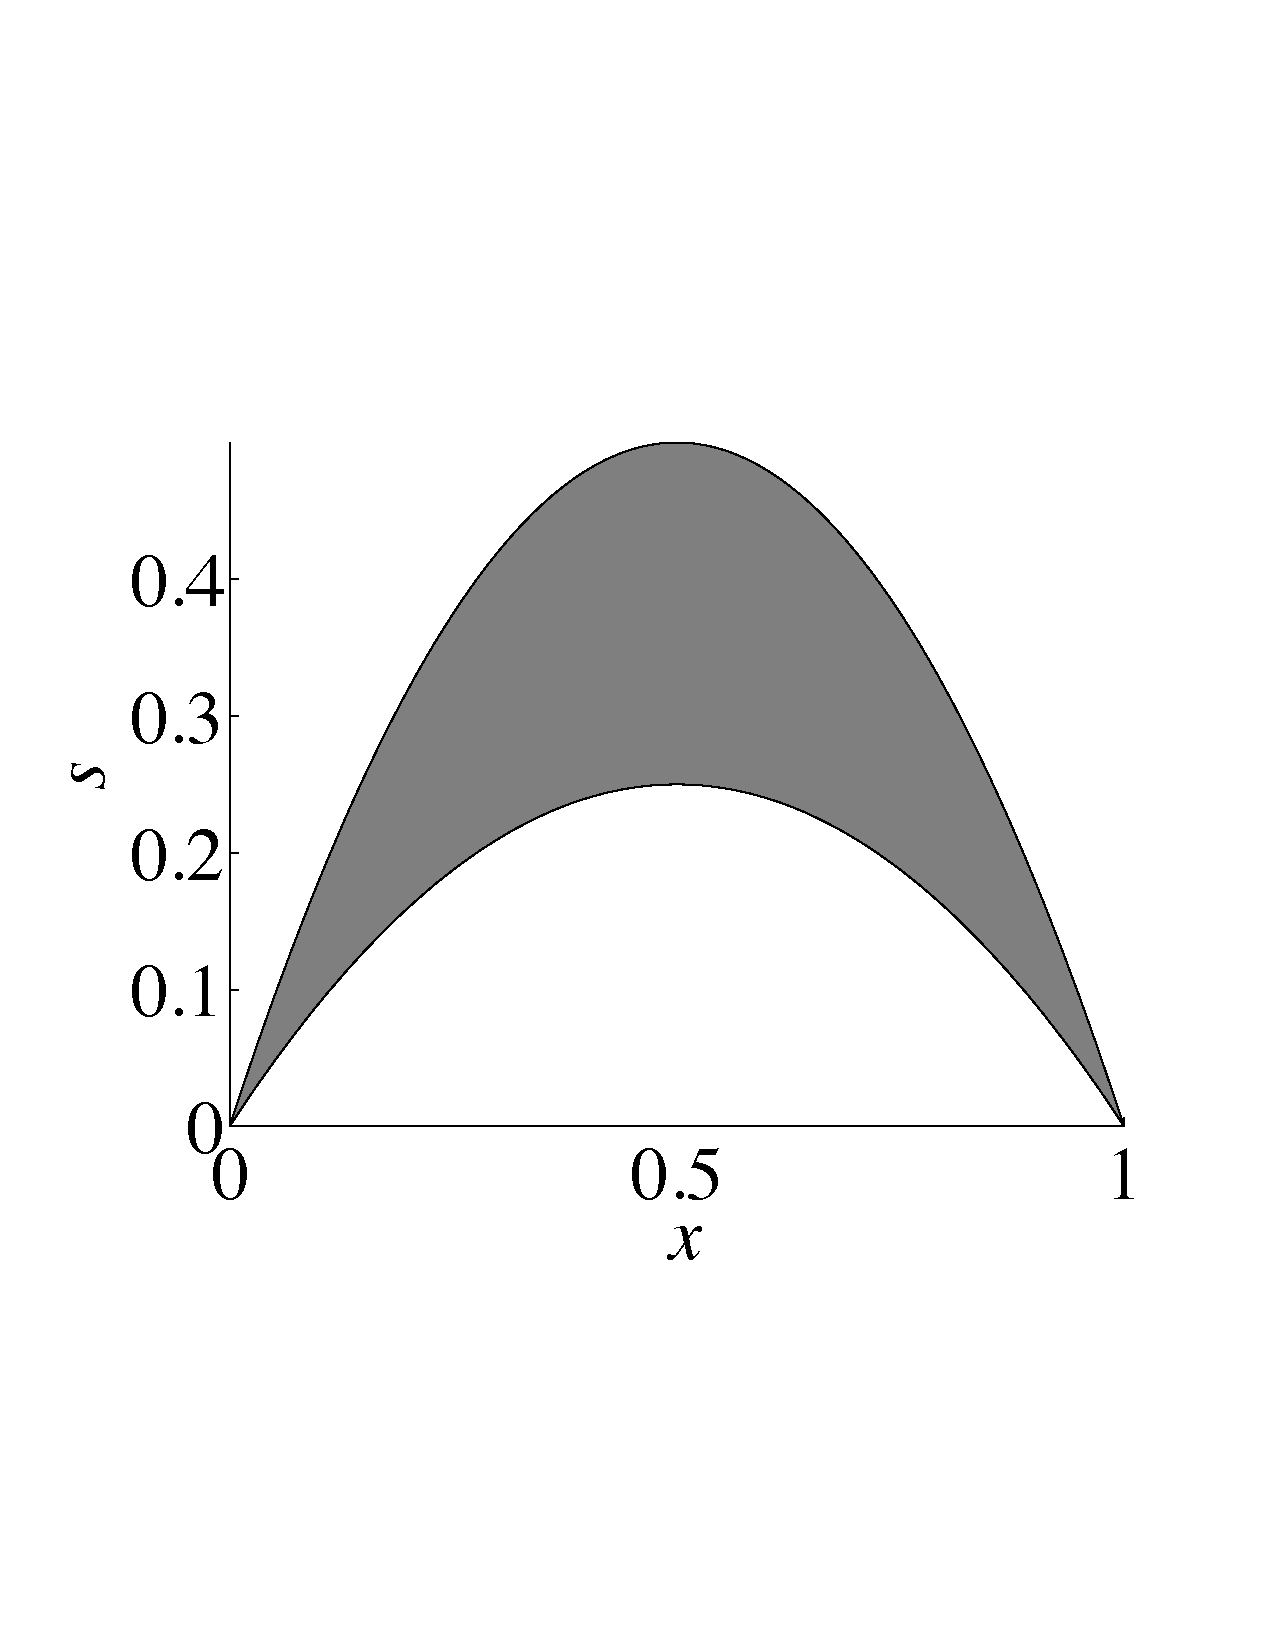
\includegraphics[width=3.5cm]{Figuras/RegionSoporteJun2013.pdf}
\part $\displaystyle \hat{s}_{\rm MMSE}= \frac{14}{9}x(1-x)$.
\part $\displaystyle \hat{s}_{\rm MAD} = \sqrt{\frac{5}{2}}x(1-x)$
\end{parts}
\end{solution}

\else

\question The joint pdf of two random variables $S$ and $X$ is given by:
$$p_{S,X}(s,x) = \left[\begin{array}{ll}
  \frac{4s}{x(1-x)}, & x(1-x)<s<2x(1-x), \quad 0<x<1 \\
  0,                 & \text{otherwise}
\end{array}  
\right. 
$$

\begin{parts}
\part Provide an approximate representation of the support of the joint distribution.
\part Obtain the estimator $\widehat S_{\text{MMSE}}$.
\part Obtain the estimator $\widehat S_{\text{MAD}}$.
\end{parts}

\begin{solution}
\begin{parts}
\part The support of the pdf is the shaded region in the following figure:

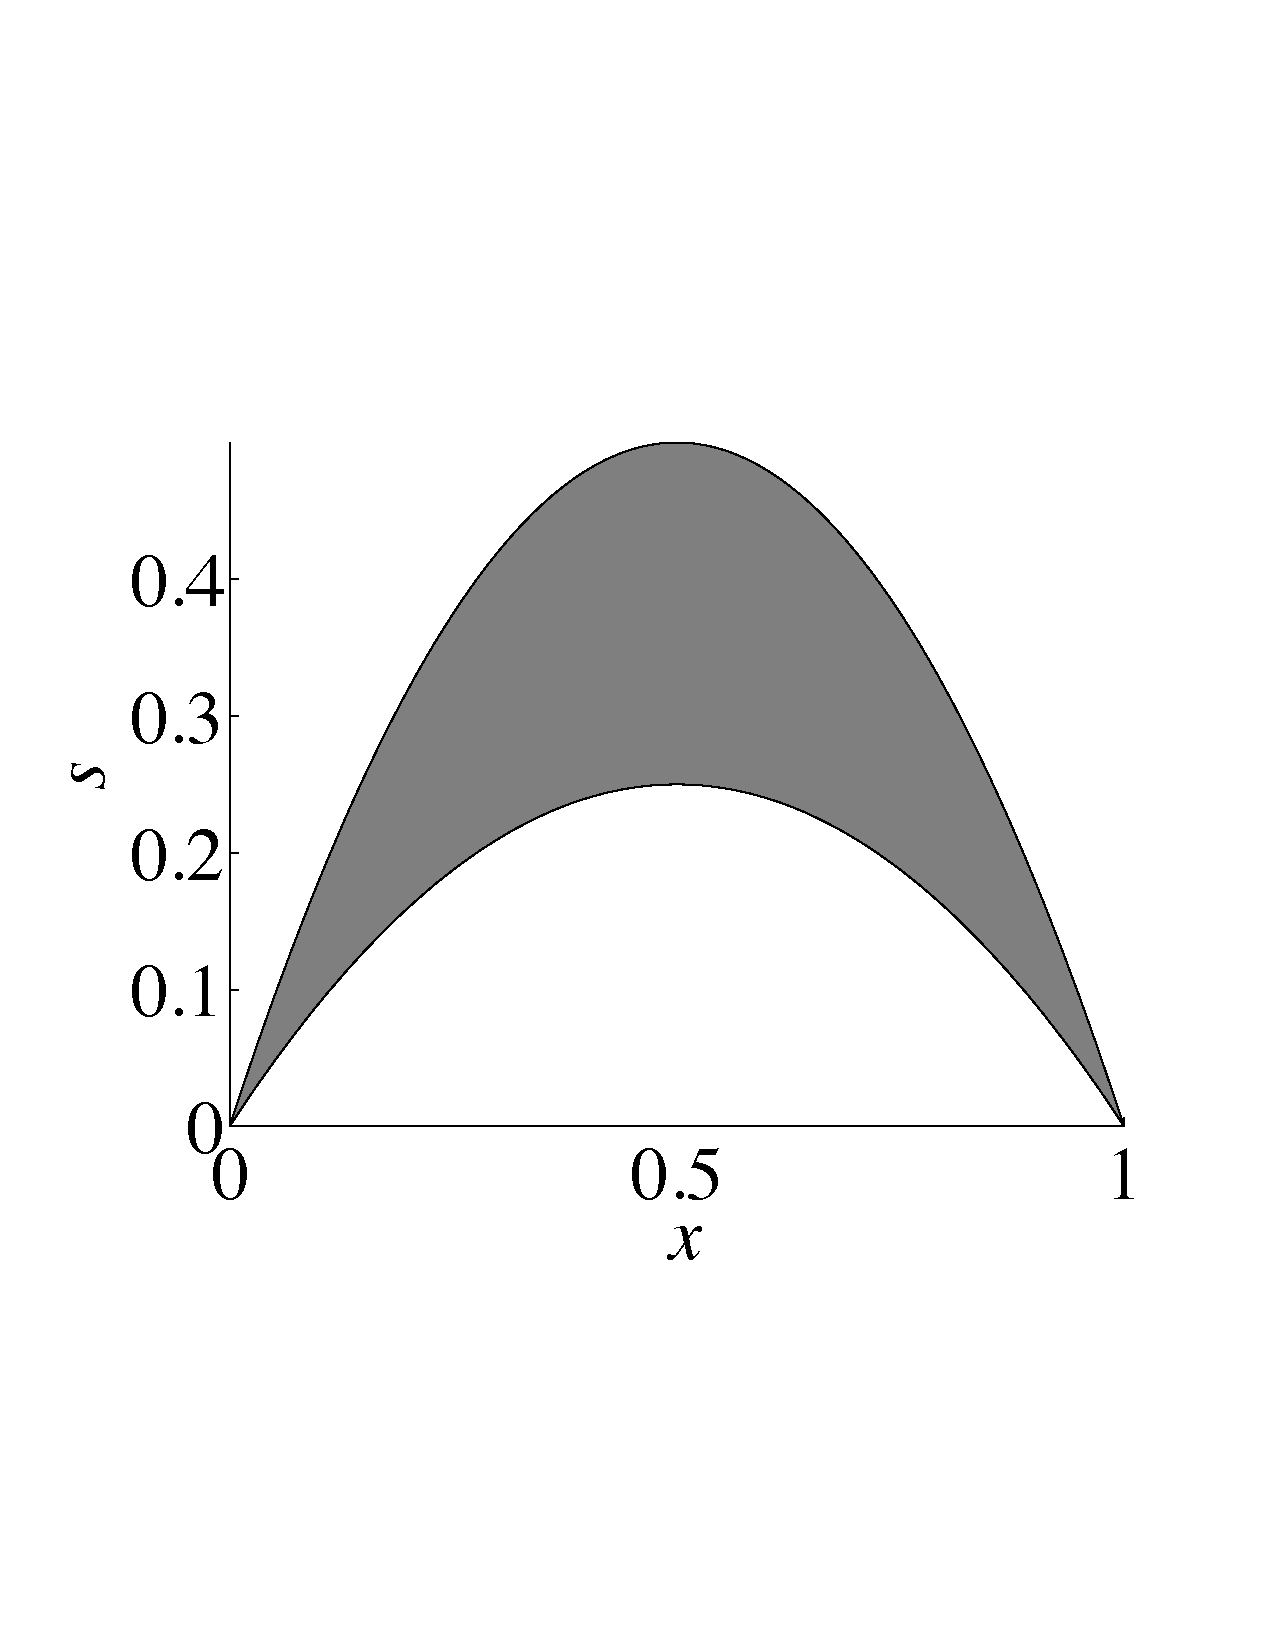
\includegraphics[width=3.5cm]{Figuras/RegionSoporteJun2013.pdf}
\part $\displaystyle \hat{s}_{\rm MMSE}= \frac{14}{9}x(1-x)$.
\part $\displaystyle \hat{s}_{\rm MAD} = \sqrt{\frac{5}{2}}x(1-x)$
\end{parts}
\end{solution}

\fi